\documentclass[preprint,3p]{elsarticle}
\usepackage{aas_macros}
\usepackage{amsmath,amssymb}
\usepackage{mathrsfs}
\usepackage{graphicx}
\usepackage{bm}
\usepackage{hyperref}

\newcommand{\mli}[1]{\mathit{#1}}
%\usepackage{epstopdf}


\begin{document}

\begin{frontmatter}

\title{Standard Candle Cosmology With Incomplete Spectroscopic Classification}
\author{A.~G. Kim\corref{cor1}}
\ead{agkim@lbl.gov}
\address{Physics Division, Lawrence Berkeley National Laboratory, 1 Cyclotron Road, Berkeley CA, USA 94720}

\begin{abstract}
\end{abstract}
\begin{keyword}
\end{keyword}
\end{frontmatter}

\section{Introduction}
A class of astronomical objects who share a common luminosity are called a standard
candle.  The relative fluxes (or magnitudes) for a set of these objects distributed in space
provide a measurement of their relative luminosity distances. These data, combined with
measurements of the standard candle redshifts, constitute a Hubble
diagram which is used to map the expansion history of the Universe.

Type~Ia supernovae (SNe~Ia) are an example of a standard candle (more precisely a standardizable
candle), whose redshift-magnitude relation provides an accurate expansion history
used to measure the Hubble Constant
\citep{2001ApJ...553...47F} and detect the accelerated expansion of the Universe
\citep{1998AJ....116.1009R, 1999ApJ...517..565P}.  SN~Ia measurements continue
to improve 
\citep{2014A&A...568A..22B} and play a critical role in probing the physics
responsible for the acceleration \citep{2013PhR...530...87W}.
Looking at the present and toward the future, SN~Ia cosmology is
a component of the Dark Energy Survey\footnote{\url{http://www.darkenergysurvey.org}} (DES),
and a science driver in the design of the
Large Synoptic Survey Telescope\footnote{\url{http://www.lsst.org}} (LSST)
and the Wide-Field InfrarRed Survey Telescope
\citep{2015arXiv150303757S}.

The information necessary to construct a Hubble diagram consists of, per object,
its classification as a
member of the standard candle class, its redshift, and its flux.  For SNe~Ia, the flux at
peak brightness is typically determined from multi-band light curves obtained from repeated
photometric observations. Traditionally, spectroscopic data is used to classify the transient
as SN~Ia through the lack of hydrogen and the presence of SiII in its spectrum,
and determine its redshift either directly through the transient spectrum or that of its host
galaxy. While the classification and redshift could be determined from the multi-band
light curves and colors of the host galaxy, the accuracy is insufficient for precision
cosmology \citep{2011ApJ...738..162S}.  Consequently spectroscopic follow-up
has played a critical role in cosmological supernova surveys.

While the large focal planes of the Dark Energy Camera (3 square degrees)
and the LSST (9.6 square degrees) open the
possibility for the photometric discovery and observation of thousands to millions
of SNe~Ia out to $z\sim1$, a corresponding multiplex advantage has not been
achieved for the 10-m
class telescopes used for the spectroscopic classification of faint discoveries:
it is unfeasible to obtain a spectrum for all SN~Ia candidates with well-measured
photometry.

Photometric supernova analysis has been proposed to  take advantage of the statistical weight imported by large numbers of supernova light curves, despite the lack of spectroscopy.
An example of such a program would proceed as follows: A rolling wide-field imaging
survey generates light curves for all transients in the survey area.  In near real-time,
a subset 
of transients from those images are selected for triggered spectroscopic observations
to obtain classifications and redshifts.  At the end of the survey, the
analysis sample is the subset of likely SN~Ia
candidates based on photometric data;  the analysis sample and its subset
with triggered spectroscopy are constructed so as to be drawn from the same parent distribution.
Spectroscopic redshifts are obtained for likely host galaxies.  The Hubble diagram of the
analysis sample is analyzed with the understanding that it may contain multiple populations.

The Sloan Digital Sky Survey-II Supernova Survey is an example of a program
that produced significant numbers of transients
with light curves but without spectroscopic typing \citep{2014arXiv1401.3317S}:
photometric SN analysis has been developed applied to these data \citep{2012ApJ...752...79H,
2013ApJ...763...88C}.   Such analyses are anticipated in the projected
supernova programs of 
DES \citep{2012ApJ...753..152B} and LSST \citep{2012arXiv1211.0310L}.

Current models used for supernova cosmology analysis account for unobserved quantities.
SNe~Ia are not standard but are ``standardizable'' candles, implying that the class may be composed of distinct subpopulations each with its own redshift-dependent rates, magnitude distributions, and secondary
observable (e.g.\ light-curve shape, color) distributions.  Bayesian hierarchical modeling is 
used to account for this extra layer of complexity  to determine characteristics of the SN~Ia population simultaneously
with the cosmology \citep{2011MNRAS.418.2308M,
2015arXiv150701602R}.  Consideration of missing classification is addressed
by
BEAMS \citep{2007PhRvD..75j3508K}, which  includes a non-Ia population in sample, whose luminosity distribution
is inferred along with the cosmology:
BEAMS was used in the analysis of SDSS-II SN data \citep{2012ApJ...752...79H}.

This article addresses the affect of missing spectroscopic typing in
a transient standard candle analysis, with the eventual goal of quantifying
requirements for the spectroscopic subsample in a broader photometric analysis.
The lack of spectroscopy leads to ambiguity in both the transient class and
in the host galaxy due to projected galaxies that appear close to the transient or
the relative low-surface brightness of the host.  The subsample with
spectroscopic typing informs the interpretation of objects lacking spectroscopy.
Differences between observed and
intrinsic distributions in a flux-limited sample can have important effects on the Hubble
diagram  (e.g.\ Malmquist bias) so are accounted for explicitly.

\section{Standard Candle}
To introduce basic model elements, this Section considers a
simplified view of SNe~Ia
as transients that are bolometric standard candles with an intrinsic random
dispersion
at peak brightness, and assumes data with negligible measurement uncertainties.
For convenience,
the transients
in this Section are  referred to as SNe~Ia.
The added complexity of correlations between absolute magnitude
and multi-band light curves, and measurement uncertainties
are discussed in
\S\ref{snIamodel:sec}. 

\subsection{Base Model}
\label{model:sec}
This Section presents a model that is used both for generating simulated data, and for analysis.
The data used to construct a Hubble diagram and the fundamental parameters of the
model used to describe those data are succinctly summarized in the notation
for the likelihood 
\begin{equation}
p(f, {{T}}_S,{{z}}_S, \theta_G|  \Omega_M, w, \theta_r,\alpha_{Ia},\sigma_{Ia}, \alpha_{\mathit{non-Ia}},\sigma_{\mathit{non-Ia}}),
\label{likelihood:eqn}
\end{equation}
whose relations are sketched in the probabilistic graphical model in Figure~\ref{toypgm:fig}.
The measurements are
\begin{itemize}
\item $f$: the flux at peak brightness, taken 
to be bolometric to facilitate the treatment of
standard candles at different redshift;
\item ${{T}}_S$, ${{z}}_S$: the spectroscopic type and redshift available for a subset of transients;
\item $\theta_{G1}$, $\theta_{G2}$: the spectroscopic redshifts of the galaxies identified
as host and neighbor from imaging.
\end{itemize}
The model parameters are
\begin{itemize}
\item $\Omega_M$, $w$: the mass density and dark-energy equation of state parameters of a flat,
constant-$w$ dark-energy cosmology;
\item $\theta_{r1}$, $\theta_{r2}$:  the parameters
that describe the redshift-dependent relative fraction of SNe~Ia and non-Ia's;
\item $\alpha_{Ia}$, $\sigma_{Ia}$, $\alpha_{\mathit{non-Ia}}$, $\sigma_{\mathit{non-Ia}}$:
the luminosity (times $4\pi$) and intrinsic dispersion for SNe~Ia and non-Ia at peak brightness.
\end{itemize}
Not listed explicitly in Eqn.~\ref{likelihood:eqn} but shown in Figure~\ref{toypgm:fig} are latent model parameters for each transient:
\begin{itemize}
\item $z$: the cosmological redshifts of the host and neighboring galaxies;
\item $T$: the class of the objects, SN~Ia or non-Ia;
\item $L$: the luminosity of the transient.
\end{itemize}
There is a  fixed parameter
\begin{itemize}
\item $\mu$: the distance modulus given the cosmological parameters and the redshift.
\end{itemize}

\begin{figure}[htbp] %  figure placement: here, top, bottom, or page
   \centering
   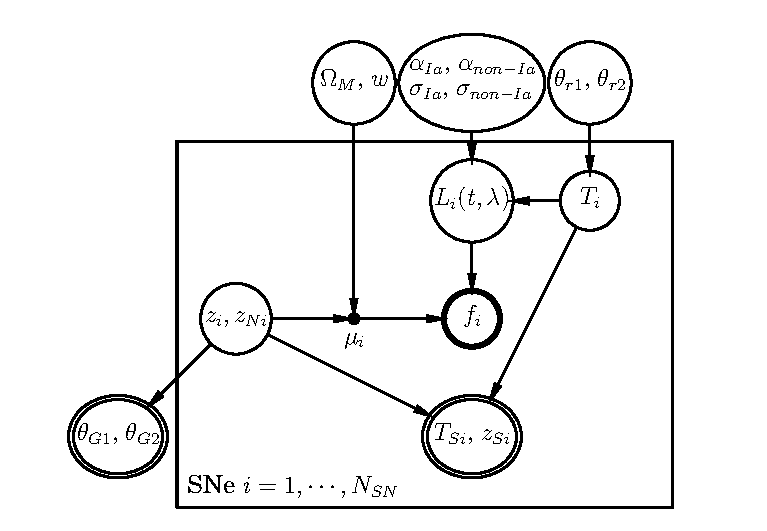
\includegraphics[width=4.5in]{/Users/akim/project/abc/results/toy_pgm.pdf} 
   \caption{Probabilistic Graphical Model for the standard candle analysis. The
   parameters include the cosmological parameters $\Omega_M$ and $w$,
   the luminosities $\alpha$ and intrinsic dispersions $\sigma$ of SNe~Ia and non-Ia's,
   and the relative fraction parameters $\theta_{r1}$ and $\theta_{r2}$.  Latent parameters
   include 
   for each transient the type $T$ and redshifts of the host and neighboring galaxies $z$ and $z_N$.  The  distance modulus $\mu$ and
   luminosity $L$ are fixed by the other parameters.  The observables include the measured
   flux $f$, spectroscopic type and redshift $T_S$ and $z_S$, and
   the inferred host and neighbor redshifts $\theta_{G1}$ and $\theta_{G2}$.
   The host and neighbor galaxies of all transients are inferred based a common galaxy catalog, 
   and so strictly are not independent from supernova to supernova.
   \label{toypgm:fig}}
\end{figure}


The transients being analyzed have passed some detection threshold
and thus are drawn from
distributions that have different shapes than the underlying population of both discovered and
non-discovered objects. A  threshold flux of $f_0$ is adopted for the detection criterion.
Otherwise, no other sample-selection criteria are assumed.

The transients are divided into
the following subsets:
{\it obs} are transients observed spectroscopically while active, from which $T_S=1$ are those typed
as SN~Ia and $T_S=0$ as non-Ia.  {\it mis} transients are not observed
spectroscopically when active.  The data from each subset have different forms for their likelihood.
The  {\it obs} sample constrains and specifies the parameter distributions of the 
parameters missing from the {\it mis} sample; both samples
are assumed to be drawn from the same underlying distribution.

\subsubsection{Likelihood for the {\it obs} set data}
\label{obs:sec}
The likelihood of data from the {\it obs} set, which has
spectroscopic observations $T_S$ and redshift
$z_S$, is described as follow.  The likelihood is
\begin{align}
p(f, {{T}}_S,{{z}}_S|  \Omega_M, w, \theta_r,\alpha_{Ia},\sigma_{Ia}, \alpha_{\mathit{non-Ia}},\sigma_{\mathit{non-Ia}}, z)  &=\sum_T
p(f, {{T}}_S,{{z}}_S, T| \ldots)\\
&= \sum_T 
p(f, {{T}}_S,{{z}}_S| T,\dots) p(T | \ldots).
\end{align}

Direct associations between model and spectroscopic redshift and type are made
\begin{align}
p(z_S|z) &= \delta(z_S-z)\\
p(T_S|T) &= \delta(T_S-T),
\label{specz:eqn}
\end{align}
so that
\begin{align}
p(f, {{T}}_S,{{z}}_S|  \ldots) &= 
p(f| T=T_S, z=z_s,\dots) p(T_S|z=z_s, \ldots).
\label{obs:eqn}
\end{align}


The first term describes the expected counts. Given the redshift
and transient type, the brightness of the underlying population
is modeled as being drawn from a standard candle
with mean luminosity $4\pi\alpha_X$ and a normal distribution in magnitude
space with intrinsic dispersion  $\sigma_X$:
\begin{equation}
f| T=T_S, z=z_S, \Omega_M, w, \theta_r, \alpha_{Ia},\sigma_{Ia}, \alpha_{\mathit{non-Ia}},\sigma_{\mathit{non-Ia}} \sim \mathcal{N}_{\ln}\left(\ln{\left(\frac{\alpha_{T_S}}{d_L^2(z_S;\Omega_M, w)}\right)}, \frac{\ln{10}}{2.5}\sigma_{T_S}\right),
\label{flux:eqn}
\end{equation}
where $\mathcal{N}_{\ln}$ is the log-normal distribution and $d_L$ is the luminosity distance.
Measurement uncertainty is taken to be negligible.
In a flux-limited survey, the pdf's for the data are truncated versions of the underlying
pdf's.
\begin{itemize}
\item For SNe~Ia  $T_S=1$:
\begin{equation}
f | T=1, z=z_S, \Omega_M, w, \alpha_{Ia},\sigma_{Ia} \sim
\frac{\mathcal{N}_{\ln}\left(\ln{\left(\frac{\alpha_{Ia}}{d_L^2(z_S;\Omega_M, w)}\right)}, \frac{\ln{10}}{2.5}\sigma_{Ia}\right)}{P_{Ia}(f > f_0)}.
\label{adusnIa:eqn}
\end{equation}
\item For non-Ia's in set $T_S=0$:
\begin{equation}
f | T=0, z=z_S, \Omega_M, w, \alpha_{\mathit{non-Ia}},\sigma_{\mathit{non-Ia}}\sim 
\frac{\mathcal{N}_{\ln}\left(\ln{\left(\frac{\alpha_{\mathit{non-Ia}}}{d_L^2(z_S;\Omega_M, w)}\right)}, \frac{\ln{10}}{2.5}\sigma_{\mathit{non-Ia}}\right)}{P_{non-Ia}(f > f_0)},
\label{adunonIa:eqn}
\end{equation}
\end{itemize}
where the normalization factor is the complementary cumulative distribution function
for the corresponding log-normal distribution that accounts for the truncated
distribution of the detected sample.
It is understood implicitly that as all objects must pass the detection threshold,
the case of $f<f_0$ is never confronted in the analysis.

The second term gives the type probability. In our model,
the underlying relative rates between SNe~Ia and non-Ia are linear in redshift,
 parameterized by the
its values at $z=0$ and $1.1 \times z_{max}$, 
\begin{equation}
\hat{\theta}_r=\theta_{r0}+z\left(\frac{\theta_{r1}-\theta_{r0}}{1.1 \times z_{max}}\right).
\label{rate:eqn}
\end{equation}
The relative rate for SN~Ia discovery for the discovered (truncated) distribution is
\begin{equation}
\theta_r=\frac{\hat{\theta}_rP_{Ia}(f > f_0)}{\hat{\theta}_{r}P_{Ia}(f > f_0) + (1-\hat{\theta}_{r})P_{non-Ia}(f > f_0)}.
\end{equation}
The spectroscopic classifications are drawn from
\begin{equation}
T_S | z=z_S, \Omega_M, w, \theta_{r0}, \theta_{r1} , \alpha_{Ia},\sigma_{Ia}, \alpha_{\mathit{non-Ia}},\sigma_{\mathit{non-Ia}} \sim \text{Bernoulli}(\theta_r).
\end{equation}
Although the underlying type distribution depends only on $ \theta_{r0}$ and $ \theta_{r1}$,  
the observed distribution does depend on the other parameters through $\theta_r$'s dependence on
the two normalization factors
$P_{X}(f > f_0)$.

%The third term is the redshift distribution of transient discoveries.
%The model takes an underlying redshift distribution of transients in the universe
%\begin{equation}
%p(z) \propto z^2.
%\end{equation}
%The redshift distribution of discovered transients is then
%\begin{equation}
%p(z) = \frac{z^2\left(\hat{\theta}_{r}P_{Ia}(f > f_0) + (1-\hat{\theta}_{r})P_{non-Ia}(f > f_0)
%\right)}{\int_{z_{min}}^{z_{max}} dz'\, z'^2\left( 
%\hat{\theta}_{r}P_{Ia}(f > f_0) + (1-\hat{\theta}_{r})P_{non-Ia}(f > f_0)
%\right)}.
%\end{equation}


\subsubsection{Likelihood for the {\it mis} set data}

Transients in the {\it mis}
set have no spectroscopic confirmation, and their data are treated as follows:
With no redshift from the transient itself, 
the redshift measurement is inferred from potential host galaxies.
In this Section, each transient is associated with two galaxies, one 
with redshift $\theta_{G1}$
that has high probability $\pi_{host}$
of being the host and the other
with redshift $\theta_{G2}$ that has probability $(1-\pi_{host})$.
In the model, the
true host redshift is $z$ and that of the interloping galaxy is $z_N$.
The likelihood for the galaxy redshifts is
\begin{equation}
P(\theta_{G1},\theta_{G2}|z, z_N) =
	\pi_{host}\delta(z-\theta_{G1})\delta(z_N-\theta_{G2}) +
	(1-\pi_{host}) \delta(z-\theta_{G2})\delta(z_N-\theta_{G1}).
\end{equation}
As with the transients, the redshifts of the host
 and neighbor galaxies are drawn from underlying distributions $p(z) \propto z^2$, $p(z_N) \propto z^2_N$.


The distribution of the underlying distribution is 
\begin{multline}
p(f, \theta_{G1}, \theta_{G2} | \Omega_M, w, \theta_r, \alpha_{Ia},\sigma_{Ia}, \alpha_{\mathit{non-Ia}},\sigma_{\mathit{non-Ia}}, z, z_N)  \\
= \sum_{T} p(f, \theta_{G1}, \theta_{G2}| T, \ldots)P(T| \ldots)\\
 =\sum_{T} p(f| T, \ldots)p(\theta_{G1}, \theta_{G2}| T, \ldots) P(T| \ldots) \\
= \sum_{T} \pi_{host} p(f| T, z=\theta_{G1} ,z_N=\theta_{G2}, \ldots) P(T| z=\theta_{G1}, ,z_N=\theta_{G2}, \ldots)  \\
 +  (1-\pi_{host}) p(f| T, z=\theta_{G2}, z_N=\theta_{G1}, \ldots) P(T| z=\theta_{G2}, z_N=\theta_{G1}, \ldots).
\label{adumis:eqn}
\end{multline}
The probabilities  for the underlying flux and
relative rate distributions
 Eqns.~\ref{flux:eqn} and \ref{rate:eqn} introduced in \S\ref{obs:sec} apply.

The data likelihood is a truncated version of the
underlying distribution: the distribution in  Eqn.~\ref{adumis:eqn} normalized by
the complementary cumulative distribution function
\begin{equation}
p(f>f_0, \theta_{G1}, \theta_{G2}|\ldots) = \int_{f_0}^{\infty} p(f, \theta_{G1}, \theta_{G2}|\ldots)df
\end{equation}
for a detection threshold of $f_0$.

\subsection{Instantiation of Simulated Data}
Two simulated data sets are realized.
The generative model of the first data set (Set 1) is
 identical to the model described in \S\ref{model:sec} with the following parameter choices:
\begin{itemize}
\item Cosmological parameters $\Omega_M=0.28$, $w=-1$.
\item Type~Ia supernovae with intrinsic dispersion $\sigma_{SNIa}=0.1$ mag.
\item Non-Ia supernovae 2 magnitudes fainter than SNe~Ia with intrinsic
dispersion $\sigma_{non-Ia}=1$ mag.
\item $z_{max}=1.4$.
\item $\theta_{r0}=0.95$, $\theta_{r1}=0.2$ for the relative fraction of SNe~Ia
at $z=0$ and $z=1.1 \times z_{max}$ respectively.
\item 2000 transients total, including discovered and non-discovered,
in the range $0.1<z<z_{max}$.
\item Detection threshold $f_0$ at approximately the mean brightness SN~Ia at $z=1$.
\item Limits of neighbor-galaxy redshifts of $0.1/1.1$ and $1.1\times z_{max}$.
\item $\pi_{host}=0.98$ for the probability of correct host-galaxy assignment.
\item Accumulated spectra for 0\%, 20\%, 60\%, and 100\% of discovered transients.
\end{itemize}

Figures~\ref{hd:fig} and \ref{hist:fig} show
the Hubble diagram 
and redshift histogram for discovered SNe~Ia and non-Ia respectively
for a realization drawn from this model.
SNe~Ia's are shown in blue and non-Ia's in red, those that fall below detection threshold
are transparent.  The solid points
represent those objects spectroscopically typed for the case of 20\% follow-up.
The green X's represent the 2\% among those without spectroscopy that
are assigned an incorrect redshift.

\begin{figure}[htbp] %  figure placement: here, top, bottom, or page
   \centering
   \includegraphics[scale=0.4]{/Users/akim/project/abc/doc/seed2.pdf}
   \includegraphics[scale=0.4]{/Users/akim/project/abc/doc/seed2_pop2.pdf}  
\caption{Hubble diagrams for a realization drawn from Set 1 (left)
and Set 2 that contains  a second non-Ia population (right).
Type~Ia's are shown in blue and non-Ia's in red, those that fall below detection threshold
are transparent.  The green X's represent the 2\% among those without spectroscopy that
are assigned an incorrect redshift.
   \label{hd:fig}}
\end{figure}

\begin{figure}[htbp] %  figure placement: here, top, bottom, or page
   \centering
   \includegraphics[scale=0.4]{/Users/akim/project/abc/doc/seed2_hist.pdf}
   \includegraphics[scale=0.4]{/Users/akim/project/abc/doc/seed2_pop2_hist.pdf}  
\caption{Histogram of redshifts of discovered SNe~Ia and non-Ia from Set 1 (left)
and Set 2  (right).
   \label{hist:fig}}
\end{figure}

The generative model for the second realized data set (Set 2)
is a perturbed version of that used to make Set 1.
A second non-Ia population is introduced with average luminosity 0.5 mag fainter
than the Ia's and with 0.25 mag dispersion.
The relative rate of the original non-Ia population relative to the second is quadratic
in redshift:
\begin{equation}
1 -\frac{0.8}{\left(1.1\times z_{max}\right)^2}z^2.
\end{equation}
A Hubble diagram realization for Set 2 is shown in Figure~\ref{hd:fig} and its redshift histogram
is in Figure~\ref{hist:fig}.  Sets 1 and 2 are realized using the same seeds:
The salient differences
between the two realizations are that a fraction of non-Ia's have absolute magnitude
based on the second population's average luminosity and intrinsic dispersion; from
that population different transients satisfy the detection threshold; spectroscopic follow-up is redistributed
for the new set that is detected.

Sets 1 and 2 share identical discovered SNe~Ia.  For reference, this pure SN~Ia
set is analyzed with 100\% spectroscopic typing. 


\subsection{Analysis Results}
The simulated data Sets 1 and 2 are analyzed using the model described
in \S\ref{model:sec}.  The generative model for Set 1 and the analysis model are 
identical, but for Set 2 they differ.
The analysis is performed using STAN 
\citep{stan-software:2015},
a probabilistic programming language for
inference of Bayesian models with Hamiltonian Monte Carlo
using the No-U-Turn sampler \citep{Homan:2014:NSA:2627435.2638586}.  Each run of the analysis
uses 24 chains each with 1000 links.  In warmup, the first half of the links are used to
determine parameters for the integration step size and the ``mass''
parameters of the Hamiltonian. The complementary
12,000 links represent draws from the model-parameter posterior.

In lieu of including data of
a pure large SN~Ia sample at low-redshift,
priors are applied to the SN~Ia absolute magnitude and intrinsic dispersion
\begin{align}
\alpha_{SNIa} & \sim \mathcal{N}_{\ln}\left(\ln\left(\alpha^0_{SNIa}\right),\frac{\ln{10}}{2.5}0.02\right)\\
\sigma_{SNIa} & \sim \mathcal{N}_{\ln}\left(\ln\left(0.1\right),0.1\right),
\end{align}
where $\alpha^0_{SNIa}$ is the true input luminosity.


The output of the analyses are presented as contours of the model
parameter pdf's for the case of 100\% spectroscopic
typing in Figure~\ref{hd:fig}, and as the mean, median, and
credible intervals of $w$ for different fractions of
spectroscopic completeness in Table~\ref{seed2:tab}.
For Set 1  the input parameters lie 
within the 68\% credible intervals of the resultant posterior despite the non-trivial appearance of
the Hubble diagram in Figure~\ref{hd:fig}.
The decrease in spectroscopic coverage leads to shifts in $w$ of 0.04 relative to the 100\%-coverage case, which is small
relative to the credible interval range of 0.281.  However, there is an
increase in parameter uncertainties, going from $\Delta w= 0.281$ to 0.309
when there is no spectroscopy; the latter is a constraining result considering that none of the
objects are directly typed and redshifted.
Relative to Set 1 with 100\% spectrosocopy,
the subset of SNe~Ia-only has a shift in the mean $w$ of 0.12
and no appreciable increase in the uncertainty of $w$.

\begin{figure}[htbp] %  figure placement: here, top, bottom, or page
   \centering
   \includegraphics[scale=0.17]{/Users/akim/project/abc/results/seed2/{contour.2000.1.0}.pdf}
   \includegraphics[scale=0.17]{/Users/akim/project/abc/results/seed2_pop2/{contour.2000.1.0}.pdf} 
\caption{Probability distribution functions of the model parameters for the case of
 100\% spectroscopy for Model 1 (left) and Model 2 (right).
    Solid lines represent the input parameters.  Dashed lines in the
   histograms are the 0.16 and 0.84 quantiles. 
   \label{contour1:fig}}
\end{figure}

\begin{table}
\centering
\begin{tabular}{|c|cc|ccc|}
\hline
Fraction Spec&$<w>$ & $w$ median &\%-ile  &$w$ range & $\Delta w$\\ \hline
\multicolumn{6}{|c|}{SN Ia only}\\ \hline
$1.00$& $-0.94 \pm 0.09$ &$-0.94$ &$0.68$ & $[-1.076, -0.801]$ & $0.275$ \\
&  &  & $0.90$ & $[-1.166, -0.718]$ & $0.448$ \\
&  &  & $0.95$ & $[-1.208, -0.682]$ & $0.525$ \\
 \hline
\multicolumn{6}{|c|}{Set 1}\\ \hline
$1.00$ &$-1.06 \pm  0.09$ &$-1.05$ &$0.68$ & $[-1.196, -0.914]$ & $0.281$ \\
&&&$0.90$ & $[-1.292, -0.826]$ & $0.466$ \\
&&&$0.95$ & $[-1.340, -0.784]$ & $0.556$ \\
\hline
$0.60$ &$-1.08 \pm  0.10$ & $-1.08$ &$0.68$ & $[-1.227, -0.933]$ & $0.293$ \\
& & &$0.90$ & $[-1.331, -0.836]$ & $0.495$ \\
& & &$0.95$ & $[-1.385, -0.787]$ & $0.598$ \\
\hline
$0.20$ &$-1.10 \pm  0.10$ & $-1.09$ &$0.68$ & $[-1.249, -0.943]$ & $0.305$ \\
& & &$0.90$ & $[-1.354, -0.851]$ & $0.502$ \\
& & &$0.95$ & $[-1.408, -0.810]$ & $0.597$ \\
\hline
$0.00$ &$-1.07 \pm  0.10$ & $-1.06$ &$0.68$ & $[-1.218, -0.909]$ & $0.309$ \\
& & &$0.90$ & $[-1.320, -0.812]$ & $0.508$ \\
& & &$0.95$ & $[-1.372, -0.770]$ & $0.602$ \\
\hline
\multicolumn{6}{|c|}{Set 2}\\ \hline
$1.00$ &$-0.94 \pm  0.09$ &$-0.94$ &$0.68$ & $[-1.078, -0.804]$ & $0.274$ \\
&&&$0.90$ & $[-1.168, -0.720]$ & $0.447$ \\
&&&$0.95$ & $[-1.214, -0.680]$ & $0.534$ \\
\hline
$0.60$ &$-1.04 \pm  0.10$ & $-1.03$ &$0.68$ & $[-1.182, -0.883]$ & $0.298$ \\
& & &$0.90$ & $[-1.285, -0.791]$ & $0.494$ \\
& & &$0.95$ & $[-1.332, -0.749]$ & $0.583$ \\
\hline
$0.20$ &$-1.10 \pm  0.10$ & $-1.09$ &$0.68$ & $[-1.247, -0.936]$ & $0.311$ \\
& & &$0.90$ & $[-1.359, -0.840]$ & $0.518$ \\
& & &$0.95$ & $[-1.413, -0.798]$ & $0.614$ \\
\hline
$0.00$ &$-1.11 \pm  0.10$ & $-1.10$ &$0.68$ & $[-1.266, -0.948]$ & $0.317$ \\
& & &$0.90$ & $[-1.375, -0.850]$ & $0.525$ \\
& & &$0.95$ & $[-1.428, -0.808]$ & $0.621$ \\
\hline
\end{tabular}
\caption{Mean, median, and credible intervals of $w$ for the SNe~Ia only,
Model 1, and Model 2 for varying
fractions of spectroscopic coverage. \label{seed2:tab}}
\end{table}

The generative model for Set 2 differs from the analysis model.
While it is expected for the input and resultant non-Ia parameters not to match, 
when there is 100\% spectroscopic coverage the posteriors of the other
parameters accommodate the input with the $w$ posterior matching
closely that of the SN~Ia-only analysis.  Unlike Model~1, which exhibits no bias
in $w$ with decreasing spectroscopy, Model~2 does have a shift in the $w$
credible region.  
The values of the mean and median values of
$w$ for both 20\% and 0\% coverage are outside the 68\%
credible region of the ideal 100\% coverage.
The Set 2 $\Delta w$ increases quicker with decreasing spectroscopy
relative to Set 1.

These results are consistent with the trivial expectation that when generative
and analysis models are identical statistically correct parameter determinations
occur, and that analysis with an incorrect non-Ia model can lead to bias.
The latter case is mitigated with complete spectroscopic typing, though then
the non-Ia's contribute little statistically to the $w$ constraints. 




\section{SN~Ia Model}
\label{snIamodel:sec}
\subsection{Base Model}
SNe~Ia are not perfect standard candles but rather are calibrated candles whose
peak brightnesses are a
function of their internal properties discerned from their colors and light-curve evolution.
Measurement uncertainty, particularly from photometric flux
calibration and galaxy photometric redshifts, can play an important role in the statistical
reach of experiments.  This Section contains a model that expands upon the one
presented in \S\ref{snIamodel:sec} to have the fidelity needed for the photometric
supernova analysis of the Dark Energy Survey and the Large Synoptic Survey Telescope.

The likelihood is written as
\begin{equation}
p(\mathit{ADU}, {{T}}_S,{{z}}_S, \theta_{S}, \theta_G |  \Omega_M, w, \theta_r,\alpha_{Ia},\sigma_{Ia}, \alpha_{\mathit{non-Ia}},\sigma_{\mathit{non-Ia}}, \theta_{Ia}, \theta_{non-Ia}, Z, g, g_N),
\label{likelihood2:eqn}
\end{equation}
whose relations are sketched in the probabilistic graphical model in Figure~\ref{pgm:fig}.

\begin{figure}[htbp] %  figure placement: here, top, bottom, or page
   \centering
   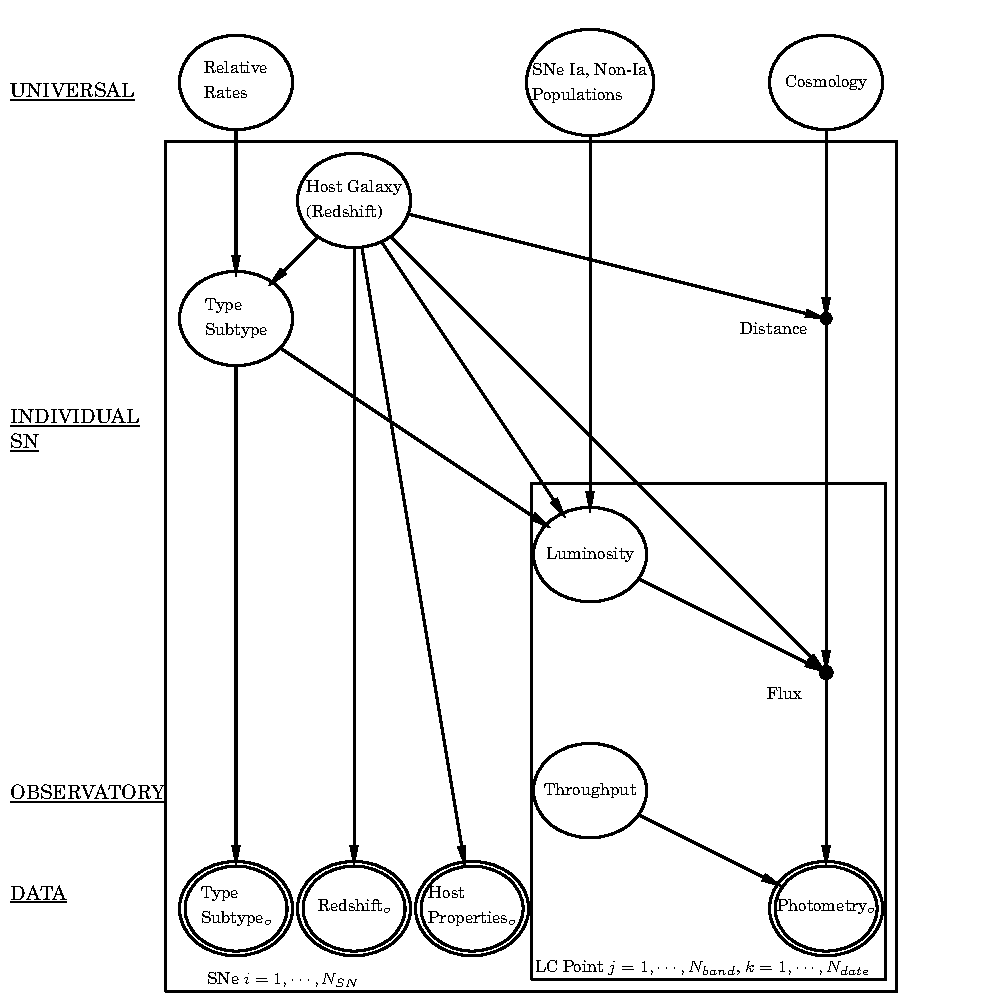
\includegraphics[width=6.5in]{/Users/akim/project/abc/results/hdpgm.pdf} 
   \caption{Probabilistic Graphical Model for the SN~Ia analysis.  
   The forward modeling
   flow goes from left to right, starting with the description of the universe, observatory,
   and data.    A transient has host galaxy $g_i$, which determines its redshift $z_i$
   and galaxy parameters $\theta_{gi}$.
   A model with parameters $\theta_\mu$ fix the distance modulus $\mu_i$.
   The transient type $T$ depends on the host-galaxy parameters  $\theta_{gi}$
   and rates $\theta_r$.   The transient
   parameters $\theta_T^X$, $\theta_{Ti}^X$ (and perhaps the host galaxy) determine the luminosity $L$.       The 
   incoming photon flux $n$, $n_g$  are then fixed
   with redshift and distance modulus.
   The instrumental transmission function $\phi$ is calibrated with data ${Z}$ andflux
   gives the expected
   counts $\overline{f}$, $\overline{f}_g$. 
   The transient has realized light curves (${ADU}$) and passes selection criteria
   through $\tau_i$ to be included in the sample.  Some transients have spectral data
   ${X}_S$.  The properties of the galaxy identified as the host galaxy is $\theta_G$. 
   \label{pgm:fig}}
\end{figure}


The new measurement that differs from  \S\ref{model:sec} is
\begin{itemize}
\item $\mathit{ADU}$: the measured counts for each photometric observation takes
the place of flux;
\end{itemize}
The new model parameters are
\begin{itemize}
\item $\theta_{Ia}$, $\theta_{non-Ia}$: the parameters for the internal diversity within SNe~Ia and
non-Ia's respectively;
\item $Z$: the parameters that describe the transmission functions, i.e.\ photometric calibration.
\end{itemize}
New latent model parameters for each transient:
\begin{itemize}
\item $\theta_{Ia,i}$, $\theta_{non-Ia,i}$: the underlying parameters that describe the transient;
\item $g$: the parameters that describe the candidate host and neighbor galaxies including redshift
is a more general replacement for $z$.
\end{itemize}
The new fixed parameters are
\begin{itemize}
\item{$z$}: the cosmological transient redshift given the host galaxy;
\item{$L$}: the luminosity of the transient with specified parameters;
\item{$f$, $f_g$}: the flux of the transient and foreground hosts;
\item{$\overline{\mathit{ADU}}$, $\overline{\mathit{ADU}}_g$}: the expected counts of the
transient and foreground galaxies.
\end{itemize}

\subsubsection{Likelihood for the obs set data}
The likelihood of data from the {\it obs} set is
\begin{equation}
p(\mathit{ADU}, {{T}}_S,{{z}}_S, \theta_S, \theta_G|  \Omega_M, w, \theta_r,\alpha_{Ia},\sigma_{Ia}, \alpha_{\mathit{non-Ia}},\sigma_{\mathit{non-Ia}}, \theta_{Ia}, \theta_{non-Ia}, Z, g, g_N).
\end{equation}
Again assuming that spectroscopy gives an unambiguous redshift, type and now adding
host-galaxy properties 
\begin{align}
p(\theta_S, \theta_G|g) &= \delta(\{\theta_S, \theta_G\} -g)
\end{align}
then
\begin{multline}
p(\mathit{ADU}, {{T}}_S,{{z}}_S, \theta_S, \theta_G|  \ldots) = \\
p(\mathit{ADU} | T=T_S, z=z_s, g=\{\theta_S, \theta_G\},  \dots) P(T_S| z= z_S , g=\{\theta_S, \theta_G\}, \ldots).
\label{obs3:eqn}
\end{multline}

The first term is the likelihood for the light curve.  The dependence of the light curve depends
on transient properties, cosmology, calibration, and the experiment.  For convenience. the
construction of the likelihood is broken up into several steps, with intermediary points
at the determination of the time and wavelength-dependent luminosity $L$,
the flux $f$, the expected counts $\overline{\mathit{ADU}}$ of the transient and background, and
finally the observed light curve $\mathit{ADU}$.  Figure~\ref{pgm:fig} shows how these
parameters are related to the intrinsic parameters and to each other.

The pdf of the luminosity $L$ can be expressed as follows:
\begin{multline}
p(L|  \theta_r,\alpha_{Ia},\sigma_{Ia}, \alpha_{\mathit{non-Ia}},\sigma_{\mathit{non-Ia}}, \theta_{Ia}, \theta_{non-Ia}, g)  \\
= \sum_T \int d\theta_{Ia}\, d\theta_{non-Ia}\, P(L, T, \theta_{Ia} \theta_{non-Ia}|\ldots) \\
= \sum_T \int d\theta_{Ia}\, d\theta_{non-Ia}\, P(L| T, \theta_{Ia} \theta_{non-Ia} \ldots) p(T,
\theta_{Ia}\, \theta_{non-Ia} | \ldots)
\end{multline}


\subsubsection{Likelihood for the mis set data}


%The likelihood for the model is
%\begin{multline}
%p(\mathit{ADU}, {{T}}_S,{{z}}_S,
%{{\theta}}_S, \theta_G, \tau, Z | g, \theta_\mu, \theta_r, \theta_T^{Ia}, \theta_{Ti}^{Ia}, \theta_T^{non-Ia}, \theta_{Ti}^{non-Ia}, \phi) = \\
%p(\theta_G|g)p(Z|\phi)p(\mathit{ADU}, {{T}}_S,{{z}}_S,
%{{\theta}}_S, \tau | g, \theta_\mu, \theta_r, \theta_T^{Ia}, \theta_{Ti}^{Ia}, \theta_T^{non-Ia}, \theta_{Ti}^{non-Ia}, \phi).
%\label{likelihood:eqn}
%\end{multline}

The simulation of data from the model presented in
and their analysis is implemented in Python and are available
on GitHub\footnote{{git@github.com:AlexGKim/abc.git}}.

\bibliographystyle{elsarticle-num} 
\bibliography{/Users/akim/Documents/alex}

\end{document}

%
%\subsubsection{SN~Ia Only}
%A classical analysis would only include confirmed SNe~Ia with a definitive
%redshift. The realization of simulated data has 415 Type~Ia supernovae.
%Results of the analysis of a pure SN~Ia sample with no
%host misclassification are presented:  Figure~\ref{contour.ia_only:fig}
%shows the posteriors for  $\Omega_M$--$w$ and Table~\ref{ia_only:tab} the
%credible equal-tailed intervals for $w$.  The true $w=-1$ is within
%the 0.58 credible interval. (Note that $w$ is the parameter
%of most interest for the experiment.)
%
%\begin{figure}[htbp] %  figure placement: here, top, bottom, or page
%   \centering
%   \includegraphics[scale=0.55]{/Users/akim/project/abc/results/{contour..ia_only.500}.pdf} \newline
%\caption{Probability distribution function for $\Omega_M$--$w$ for only SNe~Ia
%   all with spectra.
%   Solid lines represent the input cosmology.  Dashed lines in the
%   histograms are the 0.16 and 0.86 quantiles. 
%   \label{contour.ia_only:fig}}
%\end{figure}
%
%\begin{table}
%\centering
%\begin{tabular}{|c|cc|}
%\hline
%\%-ile & $w$ range & $\Delta w$\\ \hline
%$0.68$ & $[-1.254, -0.975]$ & $0.279$ \\
%$0.90$ & $[-1.347, -0.889]$ & $0.458$ \\
%$0.95$ & $[-1.396, -0.846]$ & $0.550$ \\
%\hline
%\end{tabular}
%\caption{Credible intervals of $w$ using the SNe~Ia only with spectroscopic
%observations.\label{ia_only:tab}}
%\end{table}
%
%\subsubsection{Full Sample: Varying Spectroscopic Completeness}
%We now turn to the full sample of SNe~Ia and non-Ia's.  Recall that our simple
%model treats the non-Ia's in the sample
%as standard candles with a large (1 mag) intrinsic dispersion.
%
%Results for the $\Omega_M$--$w$ posterior for the
%case of 40\%, 70\%, and 100\% spectroscopic completeness
%are shown in Figures~\ref{contour.200:fig}, \ref{contour.350:fig}, and
%\ref{contour.500:fig} respectively.
%The credible intervals
%of $w$ for are given in Table~\ref{compare:tab}, with
%the input $w=-1$ within the 0.65, 0.49, and 0.47  intervals
%respectively.
%
%\begin{figure}[htbp] %  figure placement: here, top, bottom, or page
%   \centering
%   \includegraphics[scale=0.40]{/Users/akim/project/abc/results/{contour.200}.pdf} 
%   \caption{Probability distribution function for $\Omega_M$--$w$ for:
%    SNe~Ia and non-Ia with 40\%  spectroscopic completeness.
%   \label{contour.200:fig}}
%\end{figure}
%
%\begin{figure}[htbp] %  figure placement: here, top, bottom, or page
%   \centering
%   \includegraphics[scale=0.40]{/Users/akim/project/abc/results/{contour.350}.pdf} 
%   \caption{Probability distribution function for $\Omega_M$--$w$ for
%    SNe~Ia and non-Ia with 70\%  spectroscopic completeness.
%   \label{contour.350:fig}}
%\end{figure}
%
%\begin{figure}[htbp] %  figure placement: here, top, bottom, or page
%   \centering
%   \includegraphics[scale=0.40]{/Users/akim/project/abc/results/{contour.500}.pdf} 
%   %\includegraphics[scale=0.55]{/Users/akim/project/abc/results/{contour.200}.pdf}    
%   \caption{Probability distribution function for $\Omega_M$--$w$ for
%    SNe~Ia and non-Ia with 100\%  spectroscopic completeness.
%   \label{contour.500:fig}}
%\end{figure}
%
%\begin{table}[htbp] 
%\centering
%\begin{tabular}{|cc|cc|}
%\hline
%\# Spectra & \%-ile & $w$ range & $\Delta$\\ \hline
%200& $0.68$ & $[-1.284, -0.991]$ & $0.293$ \\
%200& $0.90$ & $[-1.385, -0.900]$ & $0.485$ \\
%200& $0.95$ & $[-1.435, -0.860]$ & $0.575$ \\
%350& $0.68$ & $[-1.243, -0.952]$ & $0.291$ \\
%350& $0.90$ & $[-1.339, -0.858]$ & $0.481$ \\
%350& $0.95$ & $[-1.390, -0.817]$ & $0.573$ \\
%500& $0.68$ & $[-1.236, -0.948]$ & $0.289$ \\
%500& $0.90$ & $[-1.336, -0.861]$ & $0.475$ \\
%500& $0.95$ & $[-1.385, -0.815]$ & $0.570$ \\
%\hline
%\end{tabular}
%\caption{Credible intervals of $w$ given different levels of spectroscopy.  \label{compare:tab}}
%\end{table}
%
%As would be expected, the better the spectroscopic completeness, the less bias
%and smaller uncertainties that are obtained.
%
%
%\section{Subsections of the Model}
%
%\subsection{Type}
%\label{type:sec}
%Since our transient sample may not consist purely of SNe~Ia, the model
%has a term of the form $P(T, G | z,\mu)$, which should account for all types of
%objects that could potentially be mistaken for Type~Ia:
%the rates and association with host galaxies are described for
%the full population of potential interlopers.
%This term is not currently well known, particularly at the highest redshifts probed by DES.
%
%An idea is to consider two types: SN~Ia and non-SN~Ia, where the latter's
%intrinsic distributions have loose priors.  Transients that have been spectroscopically
%classified as non-Ia will provide the strongest leverage in constraining the
%contamination: this subset must be unbiased or properly weighted
%relative to the underlying population that constitutes the Hubble diagram.
%Running the model on a pure sample of SNe~Ia can have benefits.
%As discussed in \S\ref{systematics:sec}, comparing these results with
%those from the full sample provides
%a test of systematics.  Alternatively, the non-Ia model may be better constrained
%with the pure sample.
%
%
%To minimize the contribution of non-Ia contamination we strive for
%a pure sample selection so that $P(T=\text{non-Ia}| \mu) \rightarrow 0$.
%
%
%\subsection{Host Matching}
%\sloppy
%The host-galaxy properties depend on the GC and the transient
%coordinates $P({z}_H, {\theta}_H | {\mathit{Gals.}}, \text{RA/Dec})$.  With a
%spectrum of the transient and the underlying background, identification of the host galaxy
%is usually straightforward.
%Otherwise, projections or ambiguous cases can result in the misidentification of
%the host.
%Other supernova surveys (e.g.\ SNLS) 
%with spectroscopically confirmed host associations (e.g.\ with
%matched transient and galaxy redshifts) that replicate the DES population
%can be used to put a prior on this probability.
%
%%An effective way of addressing this term is to
%%analyze the supernovae assuming a correct host match, and
%%experimentally determine $P(\text{mismatch} )$ and
%%$\left. \langle {\mu}-\mu(z)\rangle \right|_{\text{mismatch}}$, $\left. \langle {z}-z \rangle \right|_{\text{mismatch}}$ and cross-terms to correct bias in the Hubble diagram. 
%
%
%% only model $T=\text{SN~Ia}$,
%%and experimentally determine $P(\text{non-Ia})$, 
%%$\left. \langle \mu-\mu_{model} \rangle \right|_{non-Ia}$, and its uncertainty for the
%%sample of non-Ia's that are discovered and misclassified as SN~Ia.
%%This measurement is achieved through spectroscopic
%%typing of a subset drawn from the populations used in the Hubble diagram.
%%The weighted bias would be added as a correction to the Hubble diagram under the assumption that all objects are SNe~Ia.
%
%
%\section{Systematic Tests}
%\label{systematics:sec}
%The Hubble diagrams of subsets of data quantify systematic uncertainty.  
%Subsets that may be expected to show evidence for systematics include:
%spectroscopically typed SNe~Ia; transients in deep (3) versus shallow (1/2) DES fields;
%transients with NIR data; splits based on host properties.
%
%A potentially more probative test is to compare the distance moduii inferred for the same
%supernovae, but reducing the amount of data considered.  A subset of DES
%transients have higher signal-to-noise, spectroscopic confirmation, and NIR coverage than
%the average transient, we can take away that extra information in calculating distance modulus
%to get $P(\mu | \mathit{data} - \mu | \mathit{data}^-, z | \mathit{data} - z | \mathit{data}^-)$.
%It is possible that differences in $\mu$s and $z$s have smaller uncertainties that the
%$\mu$ and $z$ alone due to common measurement uncertainties. 
%
%
%
%Generically ${{T}}$ can describe sample selection.  I choose to focus
%on objects typed as SN~Ia, rather than  all discovered transients, not just those typed as SN~Ia. 
%The non-Ia transient population has significant model uncertainty and the information they impart on the expansion history is weak:  I anticipate it is cleaner to limit ourselves to
%modeling discoveries we think are SN~Ia. This restriction does not obviate the need
%to consider non-Ia contamination in the sample, rather
%we only need to model non-Ia's
%that are mistaken for Ia and not all discovered transients. 

